\documentclass[]{article}
%opening
\title{Monte Carlo simulation of an optimized design}
\author{T.B. van der Woude}
%% Main packages in the document --- Some are imported later in the class file
\RequirePackage{mathtools}  % Mathematical tools to use with amsmath
\RequirePackage{amssymb}    % Extended symbol collection
\RequirePackage{siunitx}    % Comprehensive (SI) units package

\RequirePackage{tabularx}   % Tabulars with adjustable-width columns
\RequirePackage{booktabs}   % Publication quality tables
\RequirePackage{longtable}  % Allow tables to flow over page boundaries
\RequirePackage{multirow}   % Create tabular cells spanning multiple rows

\RequirePackage{graphicx}   % Enhanced support for images
\RequirePackage{float}      % Improved interface for floating objects
\RequirePackage[labelfont=bf,footnotesize]{caption} % Captions
% \RequirePackage[labelfont=bf,justification=centering,footnotesize]{caption} % Captions
\RequirePackage{subcaption} % Support for sub-captions
\RequirePackage{pdfpages}   % Include PDF documents

\RequirePackage[pdfusetitle,hidelinks]{hyperref} % Extensive support for hypertext
\RequirePackage[noabbrev]{cleveref} % Intelligent cross-referencing
\RequirePackage{xcolor}     % Driver-independent color extensions
\RequirePackage{tikz}       % Create PostScript and PDF graphics
\RequirePackage{xspace}     % Define commands that appear not to eat spaces
\RequirePackage{microtype}  % Refinements towards typographical perfection

\RequirePackage{geometry}   % Customize document dimensions
\RequirePackage{titlesec}   % Select alternative section titles
\RequirePackage{titletoc}   % Alternative headings for toc
\RequirePackage{fancyhdr}   % Control of page headers and footers
\RequirePackage{enumitem}   % Control layout of itemize, enumerate, description
\RequirePackage{etoolbox}   % Toolbox of programming facilities
\RequirePackage{iftex}      % Adds if-else statements to support multiple compilers
\RequirePackage{datetime}   % Change format of \today
\DeclareSIUnit\angstrom{\text{Å}}

\begin{document}
	
	\maketitle
	
	In this document, the results of an additional McStas simulation of an optimized instrument are presented. This simulation was performed after writing the report, so it is not included there. This optimized instrument has parameters $\lambda_0 = \SI{3.11}{\angstrom}$, $L_1 = \SI{3.41}{\meter}$, $L_2 = \SI{2.55}{\meter}$ and $L_s = \SI{1.27}{\meter}$. Foil flippers are used to modulate the beam and a pyrolytic graphite monochromator with $\Delta\lambda/\lambda_0 = 0.01$ is assumed. The simulated source correspondingly has FWHM $\Delta\lambda = 0.01\lambda_0$. The simulated detector has dimensions $33 \times 33 ~\unit{\milli\meter}$ and the beam has dimensions $30 \times 30 ~\unit{\milli\meter}$. The beam is focussed at the central $30 \times 30 ~\unit{\milli\meter}$, which gives an effective detector height of $h_e = \SI{30}{\milli\meter}$. The sample has thickness $t$, and a width and height of $60 \times 60 ~\unit{\milli\meter}$. To keep scattering power $\tau = \Sigma t$ reasonable, the $t$ values listed in Table \ref{tab:sample-thickness} are used. The remaining sample parameters take values $\phi = 0.015$, $\Delta\rho = \SI{1.8e10}{\centi\meter}^{-2}$ and are the same in each case. Otherwise, the simulations and instrument setup are as described in the main report. Figure \ref{fig:simulation-plot-FOIL2-PG-B-log} shows the computed $P_{exp}(\delta)$ values together with analytical $P(\delta)$ curves. Figure \ref{fig:simulation-plot-FOIL2-PG-B-lin} shows the same values and curves on a linear scale.
	\begin{table}[h!]
		\centering
		\begin{tabular}{c|cc}
			\toprule
			$R ~[\unit{\nano\meter}]$  & $t ~[\unit{\milli\meter}]$& $\tau~[\unit{\meter^3}]$ \\
			\midrule
			\num{50} & \num{20} & \num{0.0695}\\
			\num{300} & \num{10} & \num{0.2086} \\
			\num{2000} & \num{3} & \num{0.4172} \\
			\bottomrule
		\end{tabular}
		\caption{Sample radius $R$ with a sample thickness $t$ chosen to keep $\tau$ approximately within the optimal range of $0.1$ and $0.8$.}
		\label{tab:sample-thickness}
	\end{table}
	\section{Discussion}
	The most striking feature of Figures \ref{fig:simulation-plot-FOIL2-PG-B-log}, \ref{fig:simulation-plot-FOIL2-PG-B-lin} is how far off the computed values of $P_{exp}(\delta)$ are when fitting a Gaussian to the visibility $V(y)$. This indicates that a Gaussian cannot describe $V(y)$ in this setting, as confirmed by inspecting the recorded intensity data. Using the RMS of $V(y)$ to estimate $P_{exp}(\delta)$ gives values very close to the expected $P(\delta)$ curves. This indicates that it is likely possible to measure samples with radii from $R = \SI{50}{\nano\meter}$ to $R = \SI{2}{\micro\meter}$ using an instrument such as described. 
	
	\begin{figure}[p]
		\centering
		\begin{subfigure}[b]{0.95\textwidth}
			\centering
			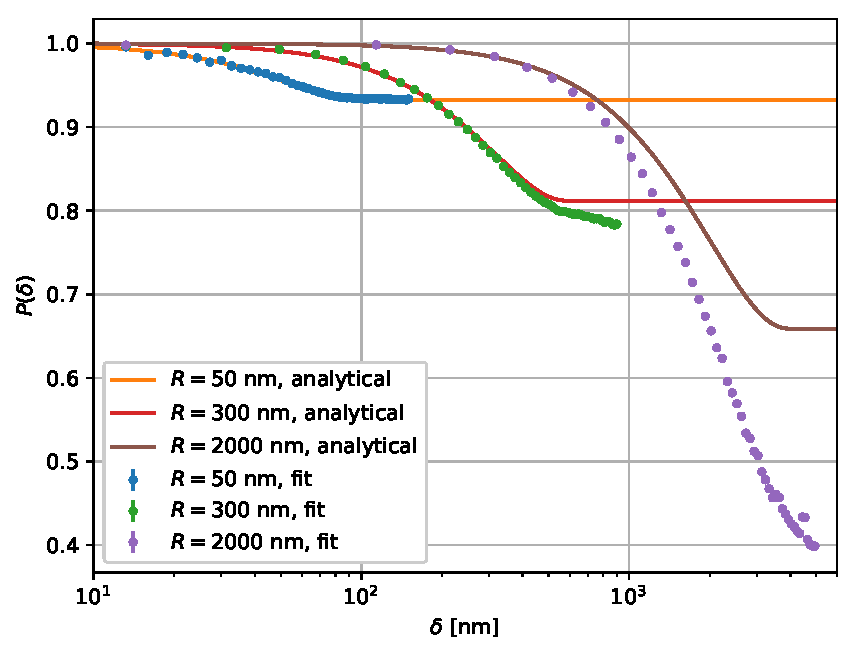
\includegraphics[width=\textwidth]{simulation-plot-gauss-FOIL2-PG-B-log}
			\caption{$P_{exp}(\delta)$ as derived using the Gauss method on a log scale.}
			\label{fig:simulation-plot-gauss-FOIL2-PG-B-log}
		\end{subfigure}
		\hfill
		\centering
		\begin{subfigure}[b]{0.95\textwidth}
			\centering
			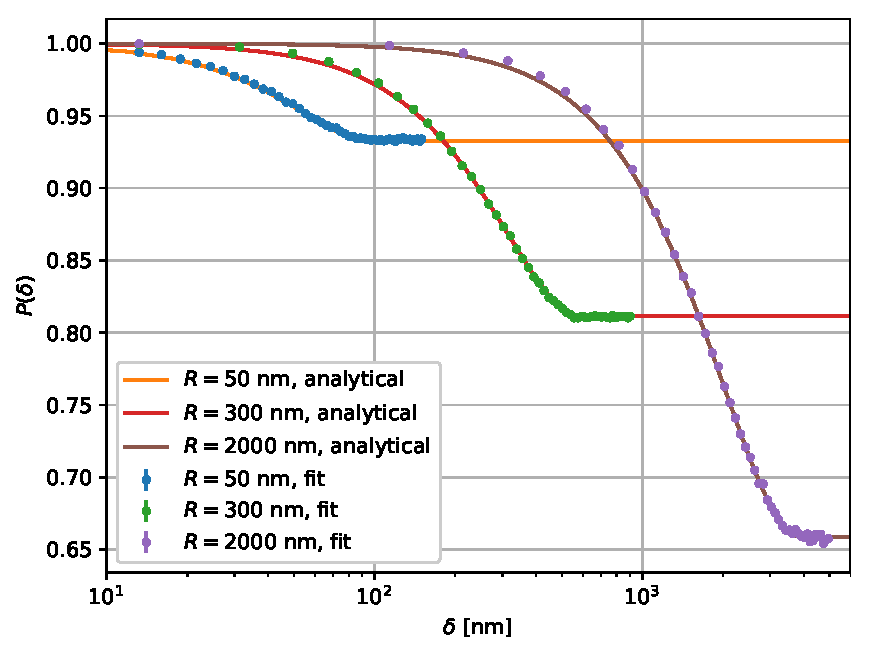
\includegraphics[width=\textwidth]{simulation-plot-rms-FOIL2-PG-B-log}
			\caption{$P_{exp}(\delta)$ as derived using the RMS method on a log scale.}
			\label{fig:simulation-plot-rms-FOIL2-PG-B-log}
		\end{subfigure}
		\hfill
		\caption{$P_{exp}(\delta)$ values derived using two analysis methods together with analytical $P(\delta)$ curves for three different samples. The instrument simulated is FOIL2 PG B. This is an instrument using foil flippers with $B_{max} = \SI{150}{\milli\tesla}$ and an effective beam height on the detector of $h_e = \SI{30}{\milli\meter}$. }
		\label{fig:simulation-plot-FOIL2-PG-B-log}
	\end{figure}
	
	\begin{figure}[p]
		\centering
		\begin{subfigure}[b]{0.95\textwidth}
			\centering
			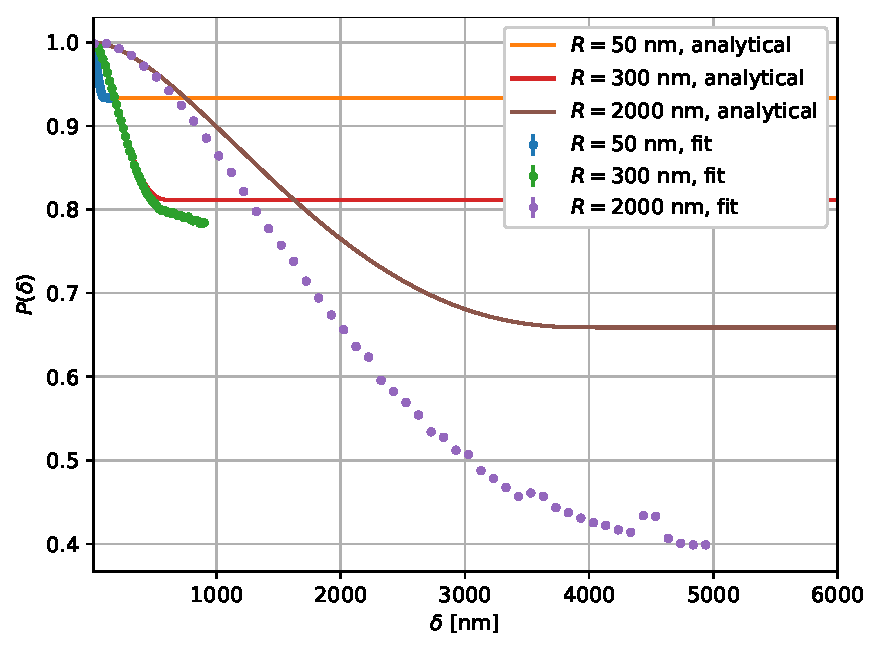
\includegraphics[width=\textwidth]{simulation-plot-gauss-FOIL2-PG-B-lin}
			\caption{$P_{exp}(\delta)$ as derived using the Gauss method on a linear scale.}
			\label{fig:simulation-plot-gauss-FOIL2-PG-B-lin}
		\end{subfigure}
		\hfill
		\centering
		\begin{subfigure}[b]{0.95\textwidth}
			\centering
			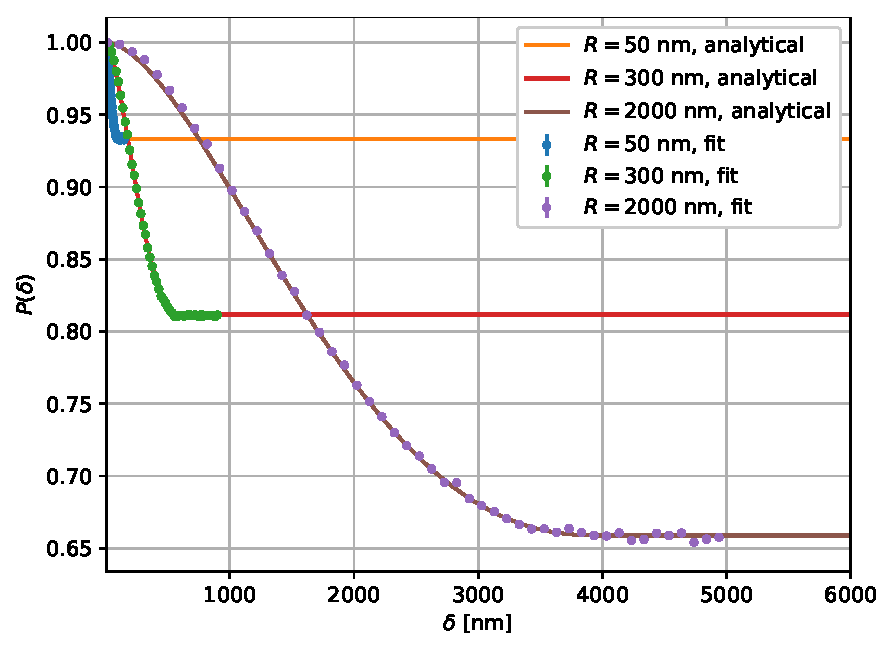
\includegraphics[width=\textwidth]{simulation-plot-rms-FOIL2-PG-B-lin}
			\caption{$P_{exp}(\delta)$ as derived using the RMS method on a linear scale.}
			\label{fig:simulation-plot-rms-FOIL2-PG-B-lin}
		\end{subfigure}
		\hfill
		\caption{The $P_{exp}(\delta)$ values and analytical $P(\delta)$ curves as shown in Figure \ref{fig:simulation-plot-FOIL2-PG-B-log} on a linear scale.}
		\label{fig:simulation-plot-FOIL2-PG-B-lin}
	\end{figure}
\end{document}
